\section{Zielsetzung}
\label{sec:Zielsetzung}

In diesem Versuch wird das Emissionsspektrum einer Kupfer Röhre analysiert, die Bragg Bedingung überprüft, und das Absorptionsspektrum für verschiedene Materialen untersucht.

\section{Theorie}
\label{sec:Theorie}

Röntgenstrahlung entsteht, wenn Elektronen aus einer Glühkathode zu einer Anode hin beschleunigt werden.
Sie lässt sich in das kontinuierliche Bremsspektrum und die charakeristische Röntgenstrahlung des Anodenmaterials aufteilen.


\noindent Trifft ein Elektron auf einen Atomkern, wird er wegen des Coulombfeldes abgebremst und verliert dabei Energie. 
Das dabei ausgesandte Photon hat genau diese Energie. Die minimale Wellenlänge des Prozesses bestimmt sich durch
\begin{equation}
\lambda_{min} = \frac{h\cdot c}{e_0 U},
\end{equation}
wobei $h$ das Plancksche Wirkungsquantum, $c$ die Lichtgeschwindigkeit, $e_0$ die Elementarladung und $U$ die Spannung ist.
Bei dem Prozess wird die kinetische Energie $E_{kin} = e_0 U$ in Strahlungsenergie $E = h\nu$ umgewandelt, mit $\nu$ als Frequenz.

\noindent Wird das Anodenmaterial ionisiert, kann ein Elektron aus einer äußeren Schale in die innere Schale, wo nun ein Elektron fehlt, fallen. Dies bechreibt das charakteristische Spektrum.
Es setzt sich aus Linien zusammen, welche mit $K_\alpha$, $K_\beta$, $L_\alpha$ bezeichnet werden. Die Buchstaben beziehen sich auf die Schale, in der der Übergang endet, und die griechischen Buchstaben beschreiben, aus welcher Schale das Elektron kommt.
Sind mehrere Elektronen in einem Atom, wird die Kernladung von den inneren Elektronen durch ihre Wechselwirkung untereinander abgeschirmt. Dementsprechend erfahren die äußeren Elektronen eine geringere Coulomb-Anziehung, und die Energie der Elektronen auf der n-ten Schale lautet
\begin{equation}
E_n = -R_\infty z_{eff}^2 \frac{1}{n^2},
\end{equation}
wobei $z_{eff} = z - \sigma$ die effektive Kernladung ist. Die Rydbergenergie wird durch $R_{\infty} = 13,6 \si{\eV}$ beschrieben und $\sigma$ ist die Abschirmkonstante.
Für die $K_\alpha$ Linie gilt
\begin{equation}
E_K{\alpha} = R_\infty (z-\sigma_1)^2 \cdot \frac{1}{1^2} - R_\infty (z-\sigma_2)^2 \cdot \frac{1}{2^2}.
\end{equation}
Die Linien sind außerdem in weiter Linien auf Grund der Feinstruktur aufgespalten.

\noindent Die Hauptwechselwirkungen zwischen Photonen mit Materie unter $1$MeV und damit der Absorption von Röntgenstrahlung sind der Comptoneffekt und der Photoeffekt. 
Ist die Photonenergie größer als die Bindungsenergie, wird der Absoprtionskoeffizient größer.
Die Absorptionskante $h \nu_{abs} = E_n - E_{\infty}$ entspricht fast komplett der Bindungsenergie eines Elektrons.
Es werden drei L-Kanten wegen der Feinstruktur beobachtet, und eine K-Kante. Berücksichtigt man jene, gilt:
\begin{equation}
E_{n,j} = -R_{\infty} \left( z_{eff,1}^2 \cdot \frac{1}{n^2} + \alpha^2 z_{eff,2}^4 \cdot \frac{1}{n^3}
\left(\frac{1}{j+ \frac{1}{2}} - \frac{3}{4n} \right) \right) ,
\end{equation}
wobei $\alpha$ die Sommerfeldsche Feinstrukturkonstante, $n$ die Hauptquantenzahl und $j$ der Gesamtdrehimpuls des
Elektrons ist.

\noindent Die Wellenlänge $\lambda$ kann man durch die Bragg-Gleichung bestimmen. Diese gilt, wenn Licht auf ein Gitter fällt, und gebeugt wird(s. Abbildung (1)).
Bei dem Glanzwinkel $\theta$ tritt konstruktive Interferenz der Strahlen auf. 
Die Gleichung lautet
\begin{equation}
  2d \sin{\Theta} = n \lambda ,
\end{equation}
wobei die Gitterkonstante $d$ bei einem LiF-Kristall $201.4 \si{\pm}$ beträgt. Der Parameter n ist außerdem die Beugungsordnung.

\begin{figure}[H]
  \centering
  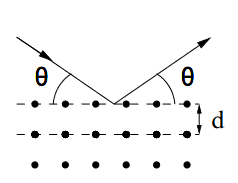
\includegraphics[height=4cm]{bragg.PNG}
  \caption{Darstellung der Bragg-Reflexion. \cite[S.2]{kent}}
\end{figure}